\documentclass[asd-beamer.tex]{subfiles}%! TEX root = asd-beamer.tex

\begin{document}
	




\begin{frame}{Test UMP unilaterale per famiglia esponenziale}\frameintoc\linkdest{UMPtestexp}
%Karlin-Rubin theorem
$X_1,\ldots,X_N$ N iid: pdf della forma $\prob{(x,\mu)}=F(x)G(\mu)\Exp{[A(x)B(\mu)]}$ e $B(\mu)$ (monotona):

UMP test (one-sided) per distinguere $H_0: \mu=\mu_0$, $H_{\mu}: \mu>\mu_0$; applico NP per $\mu_0$ e $\mu$, MP test ha la forma

\[\frac{F^N(x)G^N(\overline{\mu})}{F^N(x)G^N(\overline{\mu}_0)}\Exp{[\sum_iA(x_i)](B(\overline{\mu})-B(\overline{\mu}_0))}\gtrless c_{\alpha}\]
$F,G>0$.
Se il likelihood ratio \'e funzione monotona (non-decrescente) di una statistica $T(\vec{X})=\sum_iA(x_i)$ e scelgo $\alpha$ e $k_{\alpha}$ tali che $\prob{[\lr{(T(x))}\geq c_{\alpha}]}=\alpha$, $\lr{(k_{\alpha})}=c_{\alpha}$,  allora la regione critica per un test UMP unilaterale $H_0$ vs $H_1$ \'e $C=\{x:T(x)\geq k_{\alpha}\}$.

\cite[5]{lrtmptumpt}; \cite[445]{inferencemukhopadhyay2000}; \cite[sec 3.6]{lehmann2006testing}
\end{frame}


\begin{wordonframe}{No UMP test for two-sided hypothesis}
%insert-fig 10.9: oneone2sides
$1+$ \'e il power per UMP test per $\theta>\theta_0$, $1-$ \'e il power per UMP test per $\theta<\theta_0$: if the size of one sided tests is $\frac{\alpha}{2}$ that of two-sided (sum of the two one-sided) is $\alpha$
\begin{figure}[!ht]
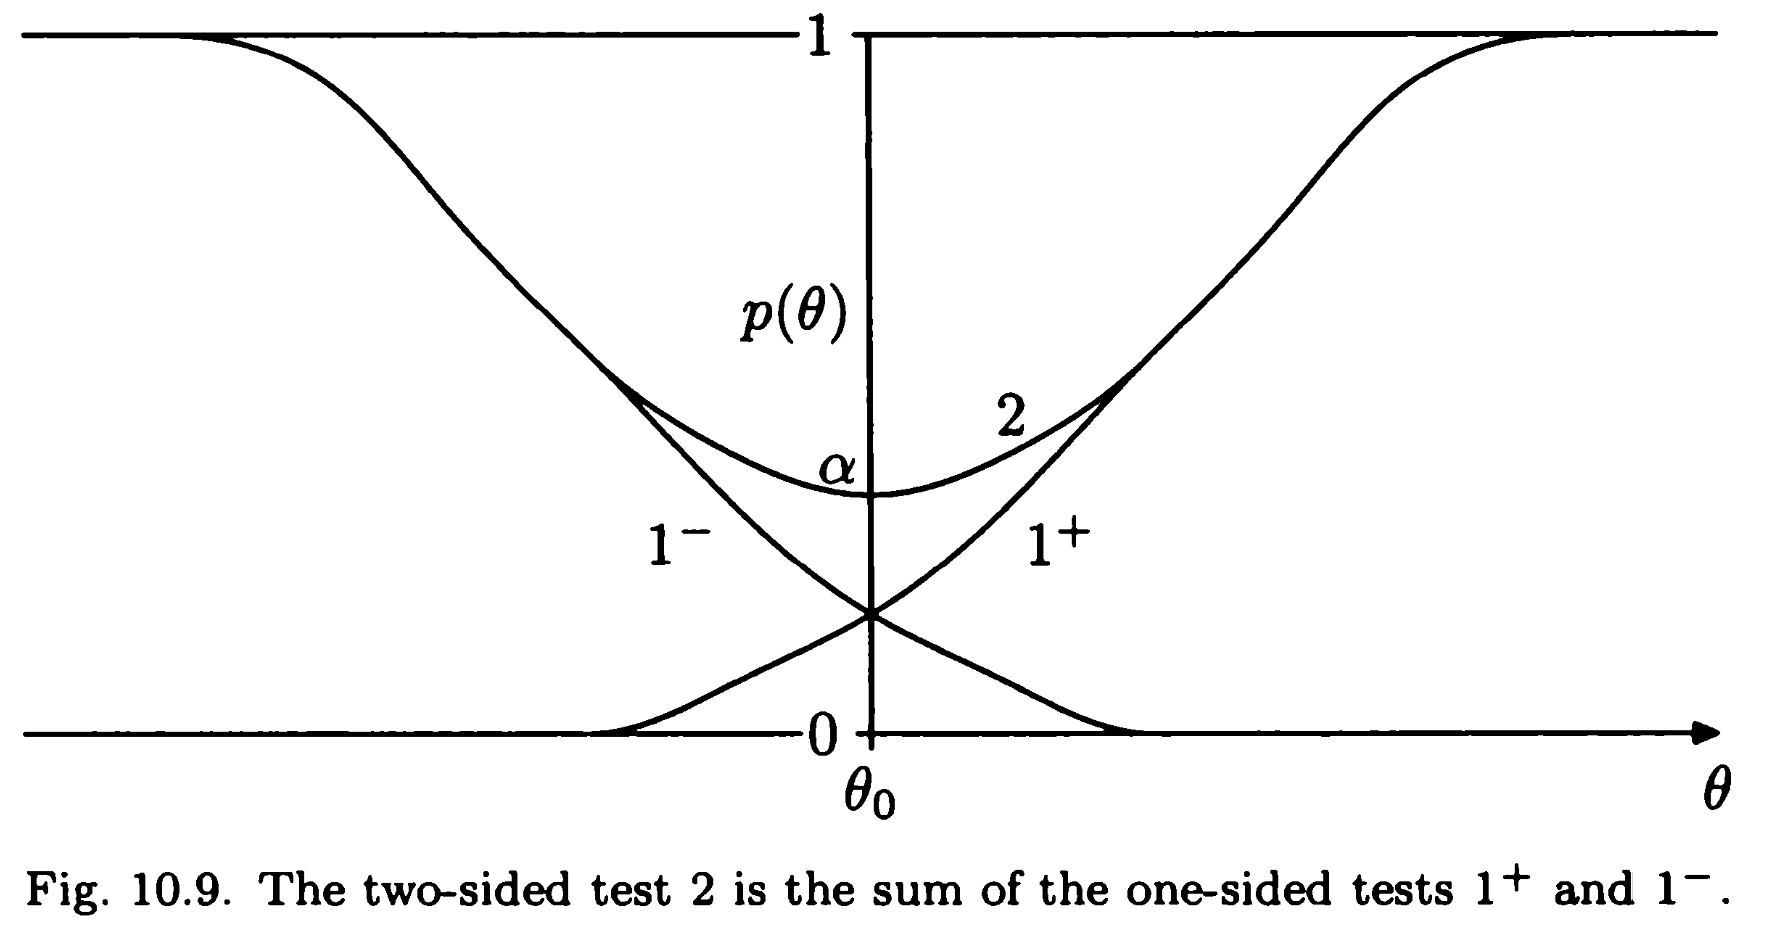
\includegraphics[trim={0cm 0cm 0 0},clip, keepaspectratio,width=0.5\textwidth]{figures/james/test/oneone2sided}
\label{fig:oneone2sided}
\end{figure}
\end{wordonframe}

\begin{frame}{Locally most powerfull (LMP) tests}\frameintoc\linkdest{LMP}
(LMP) (Se non esiste UMP test) Se ho bisogno di massima sensibilit\'a vicino alla soglia: $1-\beta$ grande nelle vicinanze di $\theta_0$: $H_0$: $\theta=\theta_0$, $H_1$: $\theta=\theta_0+\Delta$, quindi $\ln{L(\vec{X},\theta_1)}\approx\ln{L(\vec{X},\theta_0)}+\Delta\PDy{\theta}{\ln{L}}|_{\theta_0}$.
Applico NP a $H_0$ vs $H_1$:
\begin{align*}
&\ln{L(\vec{X},\theta_1)}-\ln{L(\vec{X},\theta_0)}\gtrless c_{\alpha} \Rightarrow \PDy{\theta}{\ln{L}}\gtrless q_{\alpha}\\
&\E{[\PDy{\theta}{\ln{L}}|_{\theta_0}]}=0,\ \E{[(\PDy{\theta}{\ln{L}})^2]}=NI
\end{align*}
score \'e asintoticamente normale Test: $\PDy{\theta}{\ln{L}}|_{\theta_0}\gtrless\lambda_{?1-\alpha}\sqrt{NI}$ (prob. rifiutare $H_0$ vera \'e $\alpha$).
\end{frame}

\begin{frame}{Likelihood ratio test (LRT)}\frameintoc\linkdest{LRT}
Sia $H_0: \vec{\theta}\in\nu$, $H_1: \vec{\theta}\in\overline{\nu}$
\begin{columns}[T]
\begin{column}{0.3\textwidth}
\begin{align*}
&H_0: \theta_i=\theta_{i0}, i=1,\ldots,r\\
&\theta_j, j=1,\ldots,s\\
&H_1: \theta_i\neq\theta_{i0}, i=1,\ldots,r\\
&\theta_j, j=1,\ldots,s
\end{align*}
\end{column}
\begin{column}{0.7\textwidth}
Regione critica: small $\lr$ is evidence against $H_0$ - critical region $\{\vec{x}:\lr{(\vec{x})}\leq k\}$ ($\prob{(\lr{(\vec{X})}\leq k_{\alpha};\theta)}\leq\alpha$, $\forall\theta\in\Theta_0$) - $\lambda$ funzione decrescente: $\lambda>\chi^2_{\alpha}(r)$.
\end{column}
\end{columns}
%\begin{block}{test statistic maximum likelihood ratio}
Test statistic maximum likelihood ratio
\begin{align*}
&\lr=\frac{\max_{\vec{\theta}\in\nu}L(\vec{X},\theta)}{\max_{\vec{\theta}\in\overline{\nu}}L(\vec{X},\theta)}=\frac{\max_{\vec{\theta}_s}L(\vec{X}|\vec{\theta}_{r0},\vec{\theta}_s)}{\max_{\vec{\theta}_r, \vec{\theta}_s}L(\vec{X}|\vec{\theta}_r,\vec{\theta}_s)},\ \lambda=-2\ln{\lr}
\end{align*}
Asymptotic pdf of $\hat{\theta}=(\hat{\theta}_r,\hat{\theta}_s)$ is $(r+s)$-D Normal with covariance matrix $\invers{I}$.
%\end{block}
	%$\alpha=\sup{\prob{(\lambda(\vec{X})\leq k;\theta\in\theta_0)}}$.
	Se $H_0$ impone r vincoli sugli $r+s$ parametri di $H_0$, $H_1$ ($d_{Alt}-d_{Nul}=(r+s)-s=r$):
\begin{align*}
&\forall\theta\in H_0:\ -2\log{\lr}\to\chi^2_{r}\\
&\forall\theta\in H_1:\ -2\log{\lr}\to\chi^2_{NC,r}\tag{non centrale}\\
&K_1=(\vec{\theta}_r-\vec{\theta}_{r0})^TI_r(\vec{\theta}_r-\vec{\theta}_{r0})\tag{par. non c.}\\
&1-\beta=\int_{\chi_{\alpha}^2(r)}^{\infty}dF_1[\chi^2(r,K_1)]\approx\int_{(\frac{r+K_1}{r+2K_1})\chi^2_{\alpha}(r)}^{\infty}dF_2[\chi^2(r+\frac{K_1^2}{r+2K_1})]\tag{power}
\end{align*}
\end{frame}

%\begin{frame}{LR test: critical region, significance level and power for continuus families of Hypotheses}
%\end{frame}

\begin{wordonframe}{Likelihood asymptotic expression and LRT}
%\begin{block}{Likelihood asymptotic expression}
Asymptotically MLE $\hat{\theta}$ attains MVB:
\begin{align*}
&\ln{L(\vec{X}|\theta)}-\ln{L(\vec{X}|\hat{\theta})}=\frac{1}{2}\PtwoDy{\theta}{\ln{L}}|_{\theta=\hat{\theta}}(\hat{\theta}-\theta)^2+O(N^{-3})\\
&\PtwoDy{\theta}{\ln{L}}|_{\theta=\hat{\theta}}\xrightarrow{N\to\infty}\E{[\PtwoDy{\theta}{\ln{L}}]}=-I_X\\
&L(\vec{X},\vec{\theta})=L(\vec{X},\vec{\theta}_r,\vec{\theta}_s)\propto\Exp{[-\frac{1}{2}(\hat{\theta}-\vec{\theta})^TI(\hat{\theta}-\vec{\theta})]}\\
&\lambda=\frac{L(\vec{X}|\theta_r,\hat{\theta}_s)}{L(\vec{X}|\hat{\theta_r},\hat{\theta}_s)}=\Exp{[-\frac{1}{2}(\hat{\theta}_r-\theta_{r0})^TI_r(\hat{\theta}_r-\theta_{r0})]}
\end{align*}
%\end{block}
%\begin{block}{Espansione in $\hat{\theta}-\theta_0$ per $\theta=\theta_0$}
Asymptotic normality: $\sqrt{n}(\hat{\theta}-\theta)\xrightarrow{d}N(0,\frac{1}{I(\theta)})$ quindi $I(\theta_0)(\hat{\theta}-\theta)^2\xrightarrow{D}\chi_1^2$.
%\end{block}
\end{wordonframe}

\begin{wordonframe}{Test of some theories with different dof}
%insert-fig 10.10
Maximum likelihood ratio for A vs generale case: $\lambda_a=\frac{L(0)}{L(d)}$, if hypothesis A is true $-2\ln{\lambda_a}$ is distributed asymptotically as $\chi^2(2)$; to test B vs general case ml ratio is $-2\ln{\lambda_a}$, distributed asymptotically as $\chi^2(1)$.
\end{wordonframe}

\begin{wordonframe}{Is data normally distributed (unknown variance)}
\begin{columns}[T]
	\begin{column}{0.55\textwidth}
$X_1,,X_N$ iid $N(\mu,\sigma^2)$, $H_0: \mu=0,\sigma^2$, $H_1: \mu\neq0,\sigma^2$.
Likelihood function is: 
\begin{equation*}
L(\mu,\sigma^2)=\frac{1}{(2\pi)\expy{N/2}\sigma^N}\exp{-\frac{1}{2}\sum^N\frac{(X_i-\mu)^2}{\sigma^2}}
\end{equation*}
Likelihood ratio:
\begin{align*}
&\lambda=(\frac{\sum^N(X_i-\exv{X})^2}{\sum_iX_i^2})\expy{N/2}\\
&\lambda\expy{2/N}=\frac{1}{1+\frac{t^2}{N-1}}\\
&t=\frac{\sqrt{N}\exv{X}}{\sqrt{\frac{1}{N-1}}\sum(X_i-\exv{X})^2}=\sqrt{N}\frac{\exv{X}}{s}
\end{align*}
Test based on $\lambda$ is equivalent to test based on two-sided t-test: the critical region correspond to small $\lambda$.
	\end{column}
	\begin{column}{0.45\textwidth}
Maximum likelihood estimators:
\begin{align*}
&H_0: \hat{\sigma}^2=\frac{1}{N}\sum_iX_i^2\\
&\max_{\sigma^2}L(0,\sigma)=\frac{\exp{-N/2}}{(2\pi)\expy{N/2}(\sum_iX_i/N)\expy{N/2}}\\
&H_1: \hat{\mu}=\exv{X},\ S^2=\frac{1}{N}\sum^N(X_i-\exv{X})^2\\
&\max_{\sigma^2}L(0,\sigma)=\frac{\exp{-N/2}}{(2\pi)\expy{N/2}(\sum_i(X_i-\exv{X})^2/N)\expy{N/2}}\\
\end{align*}
	\end{column}
\end{columns}

\end{wordonframe}

\begin{wordonframe}{Test whether Poissonian data have same mean}
$X_1,,X_n$ iid RV poissonian with mean $\mu_i$. $H_0: \mu_1=\mu_2=\ldots=\mu$, $H_1: \mu_i$; MLE and likelihood ratio:
\begin{align*}
&L(\mu_1,\ldots,\mu_N)=\prod_i\exp{-\mu_i}\frac{\mu_i^{X_i}}{X_i!}\\
&H_0: \hat{\mu}=\exv{X},\ \max_{\mu}L(\mu)=\frac{\exp{N\exv{X}}\exv{X}\expy{N\exv{X}}}{\prod_iX_i!}\\
&H_1: \hat{\mu}_i=X_i,\ \max_{\mu_i}L(\mu_1,\ldots,\mu_N)=\exp{N\exv{X}}\exv{X}\expy{N\exv{X}}\prod_iX_i\expy{X_i}/X_i!\\
&\lambda=\frac{\exv{X}\expy{N\exv{X}}}{\prod_iX_i\expy{X_i}}
\end{align*}
Si ritrova la statistica $\sum_i^N(X_i-\exv{X})^2/\exv{X}$ (asintotic. come $\chi^2(N-1)$) considerando $X_i=\exv{X}+\delta_i$:
\begin{align*}
&\ln{\lambda}=N\exv{X}\ln{\exv{X}}-\sum_i(\exv{X}+\delta_i)\ln{\exv{X}}-\sum_i(\exv{X}+\delta_i)(\frac{\delta_i}{\exv{X}}\\
&-\frac{\delta_i^2}{2\exv{X}^2}+\ldots)
\end{align*}
\end{wordonframe}

\begin{wordonframe}{Max power test in intervallo}
\begin{itemize}
\item \'E possible espansione L in intervallo?
\item Metodo empirico del LR. Uso stimatore ML $\hat{\mu}$: $t_{NP}=\frac{L(H_0)}{L(H_{\mu})}$. Introduco $\lambda=2\log{\frac{\sup_{\mu}}{L(\mu_0)}}$; Ipotesi complesse: $H_0: p(x;\mu_0,\nu)$ $H_{\mu}: p(x;\mu,\nu)$, $\prob{(\lambda)}\to \chi^2_{\dim{\mu-\nu}}$
\end{itemize}
\end{wordonframe}

\end{document}
